\documentclass[journal=jpcbfk,manuscript=article]{achemso}

%%%%%%%%%%%%%%%%%%%%%%%%%%%%%%%%%%%%%%%%%%%%%%%%%%%%%%%%%%%%%%%%%%%%%
%% Place any additional packages needed here.  Only include packages
%% which are essential, to avoid problems later. Do NOT use any
%% packages which require e-TeX (for example etoolbox): the e-TeX
%% extensions are not currently available on the ACS conversion
%% servers.
%%%%%%%%%%%%%%%%%%%%%%%%%%%%%%%%%%%%%%%%%%%%%%%%%%%%%%%%%%%%%%%%%%%%%
\usepackage[version=3]{mhchem} % Formula subscripts using \ce{}
\usepackage[T1]{fontenc}       % Use modern font encodings

%%%%%%%%%%%%%%%%%%%%%%%%%%%%%%%%%%%%%%%%%%%%%%%%%%%%%%%%%%%%%%%%%%%%%
%% If issues arise when submitting your manuscript, you may want to
%% un-comment the next line.  This provides information on the
%% version of every file you have used.
%%%%%%%%%%%%%%%%%%%%%%%%%%%%%%%%%%%%%%%%%%%%%%%%%%%%%%%%%%%%%%%%%%%%%
%%\listfiles

%%%%%%%%%%%%%%%%%%%%%%%%%%%%%%%%%%%%%%%%%%%%%%%%%%%%%%%%%%%%%%%%%%%%%
%% Place any additional macros here.  Please use \newcommand* where
%% possible, and avoid layout-changing macros (which are not used
%% when typesetting).
%%%%%%%%%%%%%%%%%%%%%%%%%%%%%%%%%%%%%%%%%%%%%%%%%%%%%%%%%%%%%%%%%%%%%
% \newcommand*\mycommand[1]{\texttt{\emph{#1}}}

%%%%%%%%%%%%%%%%%%%%%%%%%%%%%%%%%%%%%%%%%%%%%%%%%%%%%%%%%%%%%%%%%%%%%
%% Meta-data block
%% ---------------
%% Each author should be given as a separate \author command.
%%
%% Corresponding authors should have an e-mail given after the author
%% name as an \email command. Phone and fax numbers can be given
%% using \phone and \fax, respectively; this information is optional.
%%
%% The affiliation of authors is given after the authors; each
%% \affiliation command applies to all preceding authors not already
%% assigned an affiliation.
%%
%% The affiliation takes an option argument for the short name.  This
%% will typically be something like "University of Somewhere".
%%
%% The \altaffiliation macro should be used for new address, etc.
%% On the other hand, \alsoaffiliation is used on a per author basis
%% when authors are associated with multiple institutions.
%%%%%%%%%%%%%%%%%%%%%%%%%%%%%%%%%%%%%%%%%%%%%%%%%%%%%%%%%%%%%%%%%%%%%
\author{Kyle A. Barlow}
\affiliation{Graduate Program in Bioinformatics, University of California San Francisco, San Francisco, California, United States of America}
\email{kb@kylebarlow.com}
\author{Shane O Conch�ir}
\affiliation[QB3]{California Institute for Quantitative Biosciences, University of California San Francisco, San Francisco, California, United States of America}
\alsoaffiliation{Department of Bioengineering and Therapeutic Sciences, University of California San Francisco, San Francisco, California, United States of America}
\author{Samuel Thompson}
\affiliation{Graduate Program in Biophysics, University of California San Francisco, San Francisco, California, United States of America}
\author{Pooja Suresh}
\affiliation{Graduate Program in Biophysics, University of California San Francisco, San Francisco, California, United States of America}
\author{James Lucas}
\affiliation{Graduate Program in Bioengineering, University of California San Francisco, San Francisco, California, United States of America}
\author{Markus Heinonen}
\affiliation{Aalto University, Department of Computer Science, Espoo, Finland}
\alsoaffiliation{Helsinki Institute for Information Technology HIIT, Helsinki, Finland}
\author{Tanja Kortemme}
\affiliation[QB3]{California Institute for Quantitative Biosciences, University of California San Francisco, San Francisco, California, United States of America}
\alsoaffiliation{Department of Bioengineering and Therapeutic Sciences, University of California San Francisco, San Francisco, California, United States of America}
\alsoaffiliation{Graduate Program in Bioinformatics, University of California San Francisco, San Francisco, California, United States of America}
\alsoaffiliation{Graduate Program in Biophysics, University of California San Francisco, San Francisco, California, United States of America}
\alsoaffiliation{Graduate Program in Bioengineering, University of California San Francisco, San Francisco, California, United States of America}
\email{kortemme@cgl.ucsf.edu}

%%%%%%%%%%%%%%%%%%%%%%%%%%%%%%%%%%%%%%%%%%%%%%%%%%%%%%%%%%%%%%%%%%%%%
%% The document title should be given as usual. Some journals require
%% a running title from the author: this should be supplied as an
%% optional argument to \title.
%%%%%%%%%%%%%%%%%%%%%%%%%%%%%%%%%%%%%%%%%%%%%%%%%%%%%%%%%%%%%%%%%%%%%
\title[]
  {Flex ddG: Rosetta ensemble-based estimation of changes in protein-protein binding affinity upon mutation}

%%%%%%%%%%%%%%%%%%%%%%%%%%%%%%%%%%%%%%%%%%%%%%%%%%%%%%%%%%%%%%%%%%%%%
%% Some journals require a list of abbreviations or keywords to be
%% supplied. These should be set up here, and will be printed after
%% the title and author information, if needed.
%%%%%%%%%%%%%%%%%%%%%%%%%%%%%%%%%%%%%%%%%%%%%%%%%%%%%%%%%%%%%%%%%%%%%
% \abbreviations{}
% \keywords{}

%%%%%%%%%%%%%%%%%%%%%%%%%%%%%%%%%%%%%%%%%%%%%%%%%%%%%%%%%%%%%%%%%%%%%
%% The manuscript does not need to include \maketitle, which is
%% executed automatically.
%%%%%%%%%%%%%%%%%%%%%%%%%%%%%%%%%%%%%%%%%%%%%%%%%%%%%%%%%%%%%%%%%%%%%
\begin{document}

%%%%%%%%%%%%%%%%%%%%%%%%%%%%%%%%%%%%%%%%%%%%%%%%%%%%%%%%%%%%%%%%%%%%%
%% The "tocentry" environment can be used to create an entry for the
%% graphical table of contents. It is given here as some journals
%% require that it is printed as part of the abstract page. It will
%% be automatically moved as appropriate.
%%%%%%%%%%%%%%%%%%%%%%%%%%%%%%%%%%%%%%%%%%%%%%%%%%%%%%%%%%%%%%%%%%%%%
\begin{tocentry}
    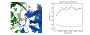
\includegraphics[width=0.8\textwidth,keepaspectratio]{figures/toc.png}
\end{tocentry}

%%%%%%%%%%%%%%%%%%%%%%%%%%%%%%%%%%%%%%%%%%%%%%%%%%%%%%%%%%%%%%%%%%%%%
%% The abstract environment will automatically gobble the contents
%% if an abstract is not used by the target journal.
%%%%%%%%%%%%%%%%%%%%%%%%%%%%%%%%%%%%%%%%%%%%%%%%%%%%%%%%%%%%%%%%%%%%%
\begin{abstract}
  Computational predicting changes in binding free energy of protein-protein interfaces after mutation allows these interactions to be designed and predicted in high throughput.
We have developed a method to predict these interface $\Delta\Delta G$s
Considering natural conformational plasticity could be helpful.
We developed a method to do this in Rosetta, using backrub based conformational sampling.
On a benchmark set of 1240 mutants, we measured performance, and were able to do better leading Rosetta methods.
On the subset of small to large, even better.
Considering flexibility was important, as a control method had a worse performance.
Averaging across more structures also improved performance.
Maching learning score function fitting also might show how the Rosetta energy function can be improved in the future.

\end{abstract}

%%%%%%%%%%%%%%%%%%%%%%%%%%%%%%%%%%%%%%%%%%%%%%%%%%%%%%%%%%%%%%%%%%%%%
%% Start the main part of the manuscript here.
%%%%%%%%%%%%%%%%%%%%%%%%%%%%%%%%%%%%%%%%%%%%%%%%%%%%%%%%%%%%%%%%%%%%%
\section{Introduction}
This is a paragraph of text to fill the introduction of the
demonstration file.  The demonstration file attempts to show the
modifications of the standard \LaTeX\ macros that are implemented by
the \textsf{achemso} class.  These are mainly concerned with content,
as opposed to appearance.

\section{Results and discussion}

\subsection{Outline}

The document layout should follow the style of the journal concerned.
Where appropriate, sections and subsections should be added in the
normal way. If the class options are set correctly, warnings will be
given if these should not be present.

\subsection{References}

The class makes various changes to the way that references are
handled.  The class loads \textsf{natbib}, and also the
appropriate bibliography style.  References can be made using
the normal method; the citation should be placed before any
punctuation, as the class will move it if using a superscript
citation style
\cite{Mena2000,Abernethy2003,Friedman-Hill2003,EuropeanCommission2008}.
The use of \textsf{natbib} allows the use of the various citation
commands of that package: \citeauthor{Abernethy2003} have shown
something, in \citeyear{Cotton1999}, or as given by
Ref.~\citenum{Mena2000}.  Long lists of authors will be
automatically truncated in most article formats, but not in
supplementary information or reviews \cite{Pople2003}. If you
encounter problems with the citation macros, please check that
your copy of \textsf{natbib} is up to date. The demonstration
database file \texttt{references.bib} shows how to complete
entries correctly. Notice that ``\latin{et al.}'' is auto-formatted
using the \texttt{\textbackslash latin} command.

Multiple citations to be combined into a list can be given as
a single citation.  This uses the \textsf{mciteplus} package
\cite{Johnson1972,*Arduengo1992,*Eisenstein2005,*Arduengo1994}.
Citations other than the first of the list should be indicated
with a star. If the \textsf{mciteplus} package is not installed,
the standard bibliography tools will still work but starred
references will be ignored. Individual references can be referred
to using \texttt{\textbackslash mciteSubRef}:
``ref.~\mciteSubRef{Eisenstein2005}''.

The class also handles notes to be added to the bibliography.  These
should be given in place in the document \bibnote{This is a note.
The text will be moved the the references section.  The title of the
section will change to ``Notes and References''.}.  As with
citations, the text should be placed before punctuation.  A note is
also generated if a citation has an optional note.  This assumes that
the whole work has already been cited: odd numbering will result if
this is not the case \cite[p.~1]{Cotton1999}.

\subsection{Floats}

New float types are automatically set up by the class file.  The
means graphics are included as follows

\begin{figure}
  As well as the standard float types \texttt{table}\\
  and \texttt{figure}, the class also recognises\\
  \texttt{scheme}, \texttt{chart} and \texttt{graph}.
  \caption{An example figure}
  \label{fgr:example}
\end{figure}

Charts, figures and schemes do not necessarily have to be labelled or
captioned.  However, tables should always have a title. It is
possible to include a number and label for a graphic without any
title, using an empty argument to the \texttt{\textbackslash caption}
macro.

The use of the different floating environments is not required, but
it is intended to make document preparation easier for authors. In
general, you should place your graphics where they make logical
sense; the production process will move them if needed.

\subsection{Math(s)}

The \textsf{achemso} class does not load any particular additional
support for mathematics.  If packages such as \textsf{amsmath} are
required, they should be loaded in the preamble.  However,
the basic \LaTeX\ math(s) input should work correctly without
this.  Some inline material \( y = mx + c \) or $ 1 + 1 = 2 $
followed by some display. \[ A = \pi r^2 \]

It is possible to label equations in the usual way (Eq.~\ref{eqn:example}).
\begin{equation}
  \frac{\mathrm{d}}{\mathrm{d}x} \, r^2 = 2r \label{eqn:example}
\end{equation}
This can also be used to have equations containing graphical
content. To align the equation number with the middle of the graphic,
rather than the bottom, a minipage may be used.
\begin{equation}
  \begin{minipage}[c]{0.80\linewidth}
    \centering
    As illustrated here, the width of \\
    the minipage needs to allow some  \\
    space for the number to fit in to.
    %\includegraphics{graphic}
  \end{minipage}
  \label{eqn:graphic}
\end{equation}

\section{Experimental}

The usual experimental details should appear here.  This could
include a table, which can be referenced as Table~\ref{tbl:example}.
Notice that the caption is positioned at the top of the table.
\begin{table}
  \caption{An example table}
  \label{tbl:example}
  \begin{tabular}{ll}
    \hline
    Header one  & Header two  \\
    \hline
    Entry one   & Entry two   \\
    Entry three & Entry four  \\
    Entry five  & Entry five  \\
    Entry seven & Entry eight \\
    \hline
  \end{tabular}
\end{table}

Adding notes to tables can be complicated.  Perhaps the easiest
method is to generate these using the basic
\texttt{\textbackslash textsuperscript} and
\texttt{\textbackslash emph} macros, as illustrated (Table~\ref{tbl:notes}).
\begin{table}
  \caption{A table with notes}
  \label{tbl:notes}
  \begin{tabular}{ll}
    \hline
    Header one                            & Header two \\
    \hline
    Entry one\textsuperscript{\emph{a}}   & Entry two  \\
    Entry three\textsuperscript{\emph{b}} & Entry four \\
    \hline
  \end{tabular}

  \textsuperscript{\emph{a}} Some text;
  \textsuperscript{\emph{b}} Some more text.
\end{table}

The example file also loads the optional \textsf{mhchem} package, so
that formulas are easy to input: \texttt{\textbackslash ce\{H2SO4\}}
gives \ce{H2SO4}.  See the use in the bibliography file (when using
titles in the references section).

The use of new commands should be limited to simple things which will
not interfere with the production process.  For example,
\texttt{\textbackslash mycommand} has been defined in this example,
to give italic, mono-spaced text: some text.

\section{Extra information when writing JACS Communications}

When producing communications for \emph{J.~Am.\ Chem.\ Soc.}, the
class will automatically lay the text out in the style of the
journal. This gives a guide to the length of text that can be
accommodated in such a publication. There are some points to bear in
mind when preparing a JACS Communication in this way.  The layout
produced here is a \emph{model} for the published result, and the
outcome should be taken as a \emph{guide} to the final length. The
spacing and sizing of graphical content is an area where there is
some flexibility in the process.  You should not worry about the
space before and after graphics, which is set to give a guide to the
published size. This is very dependant on the final published layout.

You should be able to use the same source to produce a JACS
Communication and a normal article.  For example, this demonstration
file will work with both \texttt{type=article} and
\texttt{type=communication}. Sections and any abstract are
automatically ignored, although you will get warnings to this effect.


%%%%%%%%%%%%%%%%%%%%%%%%%%%%%%%%%%%%%%%%%%%%%%%%%%%%%%%%%%%%%%%%%%%%%
%% The "Acknowledgement" section can be given in all manuscript
%% classes.  This should be given within the "acknowledgement"
%% environment, which will make the correct section or running title.
%%%%%%%%%%%%%%%%%%%%%%%%%%%%%%%%%%%%%%%%%%%%%%%%%%%%%%%%%%%%%%%%%%%%%
\begin{acknowledgement}
  The authors acknowledge our sources of funding: XX
\end{acknowledgement}

%%%%%%%%%%%%%%%%%%%%%%%%%%%%%%%%%%%%%%%%%%%%%%%%%%%%%%%%%%%%%%%%%%%%%
%% The same is true for Supporting Information, which should use the
%% suppinfo environment.
%%%%%%%%%%%%%%%%%%%%%%%%%%%%%%%%%%%%%%%%%%%%%%%%%%%%%%%%%%%%%%%%%%%%%
\begin{suppinfo}
% A listing of the contents of each file supplied as Supporting Information
% should be included. For instructions on what should be included in the
% Supporting Information as well as how to prepare this material for
% publications, refer to the journal's Instructions for Authors.

% The following files are available free of charge.
% \begin{itemize}
% \item Filename: brief description
% \item Filename: brief description
% \end{itemize}

Supplementary figures:
\begin{itemize}
\item \cref{tab:table-mult}
\item \cref{fig:steps-v-corr}
\item \cref{tab:table-versions}
\item \cref{fig:structs-v-corr-id-zemu-12-60000-rscript-validated-t14}
\item \cref{fig:structs-v-corr-WildTypeComplex-ddg-monomer-16-003-zemu-2}
\item \cref{fig:wildtypecomplex-scores-complete}
\item \cref{fig:spear-corr-rmsd-error}
\item \cref{fig:t14-mean-ensemble-error}
\end{itemize}

\subimport*{figs-and-tables/}{table-mult}
\subimport*{figs-and-tables/}{steps-v-corr}
\subimport*{figs-and-tables/}{table-versions}
\subimport*{figs-and-tables/}{structs-v-corr-id-zemu-12-60000-rscript-validated-t14}
\subimport*{figs-and-tables/}{structs-v-corr-WildTypeComplex-ddg-monomer-16-003-zemu-2}

\begin{figure}
  \includegraphics[width=\textwidth,keepaspectratio]{figures/wildtypecomplex-scores-complete.pdf}
  \caption{
    Contour plot showing the effect of backrub sampling on the average wild-type complex score, for varying numbers of averaged models.
  } \label{fig:wildtypecomplex-scores-complete}
\end{figure}

\begin{figure}
  \includegraphics[width=\textwidth,keepaspectratio]{figures/t14-mean-ensemble-error.pdf}
  \caption{
    Mean backrub ensemble RMSD vs. backrub steps.
  } \label{fig:t14-mean-ensemble-error}
\end{figure}

\begin{figure}
  \includegraphics[width=\textwidth,keepaspectratio]{figures/t14-spear-corr.pdf}
  \caption{
    Scatter plot showing the average Spearman correlation of ddG prediction error v. mean backrub ensemble RMSD, v. backrub steps.
  } \label{fig:spear-corr-rmsd-error}
\end{figure}
\end{suppinfo}

%%%%%%%%%%%%%%%%%%%%%%%%%%%%%%%%%%%%%%%%%%%%%%%%%%%%%%%%%%%%%%%%%%%%%
%% The appropriate \bibliography command should be placed here.
%% Notice that the class file automatically sets \bibliographystyle
%% and also names the section correctly.
%%%%%%%%%%%%%%%%%%%%%%%%%%%%%%%%%%%%%%%%%%%%%%%%%%%%%%%%%%%%%%%%%%%%%
\bibliography{references}

\end{document}
